\label {fs-short-experiments}

\begin{figure*}[t!]
    \begin{subfigure}[b]{0.31\textwidth}
            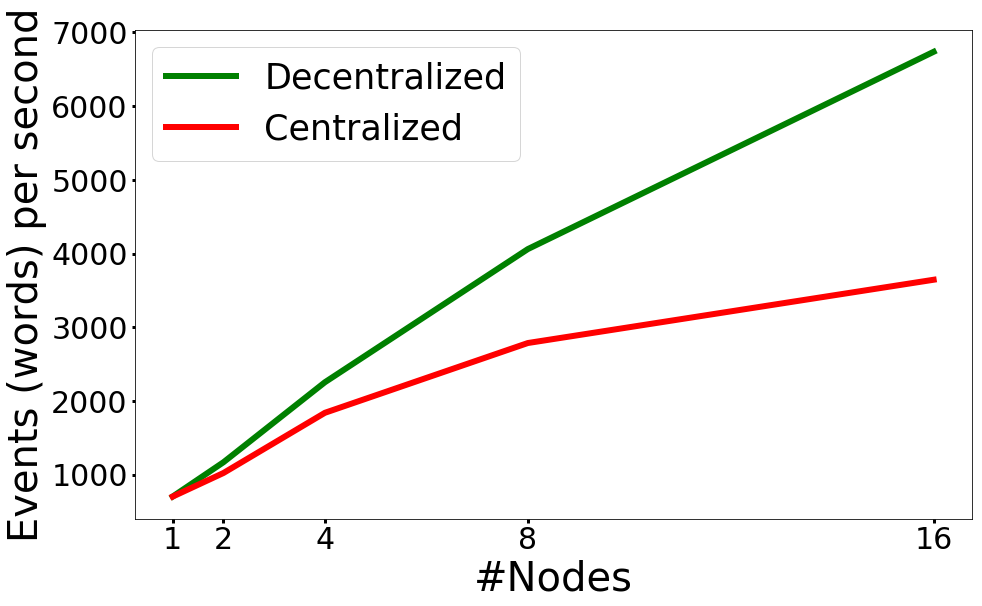
\includegraphics[width=\linewidth]{pics/throughput}
            \caption{Throughput for centralized and decentralized approaches}
            \label{throughput}
    \end{subfigure}%
    \hspace{5mm}
    \begin{subfigure}[b]{0.31\textwidth}
            \includegraphics[width=\linewidth]{pics/detection_rate}
            \caption{Change detection speed for round robin and hash partitionings}
            \label{detection_rate}
    \end{subfigure}%
    \hspace{5mm}
    \begin{subfigure}[b]{0.31\textwidth}
            \includegraphics[width=\linewidth]{pics/decision_making.png}
            \caption{A comparison between decision making approaches}
            \label{decision_making}
    \end{subfigure}%
    \caption{Results of preliminary experiments}
\end{figure*}


\indent

{\bf Setup.} We conducted several experiments to demonstrate that the proposed problem statement is reasonable and to determine basic directions towards a solution. As a validation task, we chose to check that frequencies of words in an input stream fit Zipf distribution. Such a stream of words can be considered as a part of word count or IDF computing pipelines. As it was mentioned above, this setup is useful for fraud detection. We used words from Wikipedia corpus as an input stream for experiments.

{\bf Throughput.} We measured the throughput of two approaches: centralized, where words are merged into a single node for validation, and decentralized. Experiments were conducted with Apache Flink on a cluster of Amazon EC2 small instances with 1 core CPU and 2GB RAM. Figure~\ref{throughput} shows that centralized method significantly limits throughput and scalability and may significantly influence the performance of the whole data flow. This result demonstrates that decentralized validation problem statement has a practical rationale.

{\bf Change detection speed.} In this experiment, we measured the duration (in input events) of change detection. A change in data was simulated using input from the generated corpus with lognormally distributed word frequencies. We compared two data partitioning methods. The first one is natural for word count and IDF computing task: each word sticks to a single node. In this case, each node processes only its own subsample of all possible words. The second approach is round robin. While it is not suitable for word count, such partitioning ensures that each word may be processed on all computational nodes. As expected, Figure~\ref{detection_rate} demonstrates that round robin provides faster detection, because simulated lognormal data is distributed among nodes in a more uniform way. This behavior means that for faster detection, it may be reasonable to reshuffle words in a round-robin manner after, e.g. IDF aggregation.

{\bf Approaches for making decisions.} This experiment demonstrates a comparison between three simple mechanisms for making a global decision about hypothesis acceptance based on local decisions of each node. The first method rejects a hypothesis if at least one node rejects it. The second technique makes the decision based on a majority vote of all nodes decisions. The last method rejects hypothesis only if all nodes rejects it. Figure~\ref{decision_making} shows a dependency between a number of nodes and the number of input elements needed to detect change for each of the proposed methods within round robin partitioning. As we can see, the choice of a method for making decision significantly affects detection speed. On the other hand, various methods may provide distinct false positive and false negative rates. The investigation of the statistical properties of methods for making a decision is an essential part of the proposed problem solution.